\documentclass{report}
\usepackage[T1]{fontenc} % Fontes T1
\usepackage[utf8]{inputenc} % Input UTF8
\usepackage[backend=biber, style=ieee]{biblatex} % para usar bibliografia
\usepackage{csquotes}
\usepackage[portuguese]{babel} %Usar língua portuguesa
\usepackage{blindtext} % Gerar texto automaticamente
\usepackage[printonlyused]{acronym}
\usepackage{hyperref} % para autoref
\usepackage{graphicx}
\usepackage{indentfirst}
\usepackage{lmodern}
\usepackage{epigraph} 
\usepackage{xskak}
\usepackage[export]{adjustbox}
\usepackage{subcaption}
\usepackage{wrapfig}
\usepackage{multirow}
\usepackage{tabularx}
\usepackage{array}


\bibliography{bibliografia}


\begin{document}
%%
% Definições
%
\def\titulo{Inteligência Artificial}
\def\data{DATA}
\def\autores{Bernardo Marujo}
\def\autorescontactos{(107322) bernardomarujo@ua.pt}
\def\versao{Versão 1}
\def\departamento{Dept. de Eletrónica, Telecomunicações e Informática}
\def\empresa{Universidade de Aveiro}
\def\logotipo{ua.pdf}
%
%%%%%% CAPA %%%%%%
%
\begin{titlepage}

\begin{center}
%
\vspace*{50mm}
%
{\Huge \titulo}\\ 
%
\vspace{10mm}
%
{\Large \empresa}\\
%
\vspace{10mm}
%
{\LARGE \autores}\\ 
%
\vspace{30mm}
%
\begin{figure}[h]
\center
\includegraphics{\logotipo}
\end{figure}
%
\vspace{30mm}
\end{center}
%
\begin{flushright}
\versao
\end{flushright}
\end{titlepage}

%%  Página de Título %%
\title{%
{\Huge\textbf{\titulo}}\\
{\Large \departamento\\ \empresa}
}
%
\author{%
    \autores \\
    \autorescontactos
}
%
\date{\today}
%
\maketitle

\pagenumbering{roman}
%%%%%%%%%%%%%%%%%%%%%%%%%%%%%%%%%%%%%%%%%%%%%%%%%%%%%%%%%%%%%%%%%%%%%%%%%%%%%%%%%%%%%%%%%%%%%%%%%%%%%%%%%%%%%%%%
%%%%%% RESUMO %%%%%%
\begin{abstract}
Este trabalho aborda o tema \textbf{Inteligência Artificial} (mais conhecida e referenciada pelo nome e sigla em inglês \ac{ai}), que está cada vez mais presente na nossa sociedade com o desenvolvimento da tecnologia. O trabalho incide na evolução da \ac{ai} ao longo dos últimos anos, na sua aplicação em áreas importantes que vão mudar o mundo como o conhecemos, o uso de \ac{ai} em robôs humanóides e nos softwares dos carros, e também dois tópicos mais específicos do uso de \ac{ai}, a ferramenta GitHub Copilot e a criação de \textit{chess engines}, programas de computador capazes de jogar xadrez. São também abordadas as consequências negativas do uso de \ac{ai}, especialmente quando se fala em robôs, que podem vir a constituir um problema grave para o ser humano no futuro.
\end{abstract}
%%%%%%%%%%%%%%%%%%%%%%%%%%%%%%%%%%%%%%%%%%%%%%%%%%%%%%%%%%%%%%%%%%%%%%%%%%%%%%%%%%%%%%%%%%%%%%%%%%%%%%%%%%%%%%%%
%%%%%% Agradecimentos %%%%%%
% Segundo glisc deveria aparecer após conclusão...
%\renewcommand{\abstractname}{Agradecimentos}
%\begin{abstract}
%Não existem agradecimentos a fazer.
%\end{abstract}


\tableofcontents
% \listoftables     % descomentar se necessário
% \listoffigures    % descomentar se necessário


%%%%%%%%%%%%%%%%%%%%%%%%%%%%%%%
\clearpage
\pagenumbering{arabic}


%%%%%%%%%%%%%%%%%%%%%%%%%%%%%%%%
%%%%%%%%%%%%%%%%%%%%%%%%%%%%%%%%%%%%%%%%%%%%%%%%%%%%%%%%%%%%%%%%%%%%%%%%%%%%%%%%%%%%%%%%%%%%%%%%%%%%%%%%%%%%%%%%
\chapter{Introdução}
\label{chap.introducao}
\section{Estrutura do documento}


Este documento está dividido em oito capítulos.
Depois desta introdução, é feita uma breve alusão aos diferentes tipos de \ac{ai}, seguindo-se dos quatro capítulos principais, onde, em cada um deles, é introduzido um aspeto diferente da utilização de \ac{ai}.
No \autoref{chap.robos} é apresentado o uso da \ac{ai} na construção de \textbf{Robôs},
no \autoref{chap.automoveis} a sua aplicação nos software dos \textbf{Automóveis}, no \autoref{chap.github} a sua aplicação numa ferramenta de ajuda a programadores chamada \textbf{GitHub Copilot}, no \autoref{chap.xadrez} a sua aplicação no desenvolvimento de \textbf{\textit{Chess Engines}}, e por último no \autoref{chap.perigos} é feita uma pequena exposição dos problemas que podem surgir derivados do uso de \ac{ai}.
Finalmente, no \autoref{chap.conclusao} são apresentadas as conclusões do trabalho.


\section{O que é \ac{ai}}

\ac{ai} significa inteligência artificial. Refere-se à capacidade de um programa, de um computador ou máquina de imitar ou replicar o comportamento humano inteligente. Isso pode incluir tarefas como resolução de problemas, aprendizado e tomada de decisões. A \ac{ai} é um campo em rápido crescimento que tem o potencial de transformar muitos setores, indústrias e aspetos das nossas vidas \cite{paper1}.


\epigraph{AI is the science of endowing programs with the ability to change themselves for the better as a result of their own experiences. }{\textit{Roger C. Schank}}


\section{Aplicação da \ac{ai} no quotidiano}

A \ac{ai} é usada para uma ampla gama de aplicações, incluindo tradução de idiomas, reconhecimento de imagem e fala e veículos autónomos. Em muitos casos, a \ac{ai} pode ser usada para automatizar tarefas que seriam demoradas ou difíceis de serem executadas por humanos, como analisar grandes conjuntos de dados ou tomar decisões complexas. A \ac{ai} também é usada em vários setores, desde saúde e finanças até agricultura e transporte.
Cada vez mais a \ac{ai} está integrada nas nossas vidas diárias, mesmo de maneiras que podemos não perceber. Por exemplo, a \ac{ai} é usada em muitos dos produtos e serviços que usamos regularmente, desde assistentes virtuais como Siri e Alexa até algoritmos de recomendação em serviços de streaming como Netflix.
À medida que o campo da \ac{ai} continua a avançar, espera-se que os usos potenciais desta tecnologia se expandam ainda mais.



\section{Como é desenvolvida \ac{ai}}

\ac{ai} é desenvolvida por meio de uma combinação de ciência da computação, matemática e engenharia. O desenvolvimento da \ac{ai} normalmente envolve a criação de algoritmos que permitem que um programa de computador ou máquina processe e analise grandes quantidades de dados para tomar decisões ou previsões. Isso pode incluir técnicas como aprendizado de máquina, em que um programa é treinado em um grande conjunto de dados e é capaz de melhorar seu desempenho ao longo do tempo. Além disso, os sistemas de \ac{ai} geralmente incorporam elementos de neuro-ciência e psicologia para modelar melhor a cognição e o comportamento humano.

A história da \ac{ai} remota à década de 1950, quando os pesquisadores começaram a explorar o conceito de máquinas que poderiam pensar e raciocinar como humanos. Um dos primeiros exemplos de \ac{ai} foi um programa chamado \textit{General Problem Solver}, desenvolvido por Herbert Simon e Allen Newell no final dos anos 1950. Este programa foi capaz de resolver problemas simples usando lógica e raciocínio, estabelecendo as bases para futuras pesquisas de \ac{ai}.

Nas décadas de 1980 e 1990, a pesquisa de \ac{ai} começou a se concentrar mais no uso de aprendizado de máquina, que envolve treinamento de algoritmos em grandes conjuntos de dados para fazer previsões ou decisões. Isso levou ao desenvolvimento de sistemas de \ac{ai} capazes de realizar tarefas como reconhecimento de imagem e fala, que se tornaram cada vez mais comuns no mundo atual.
\footnote{Roger C. Schank; What Is AI, Anyway? \cite{paper1}}

%%%%%%%%%%%%%%%%%%%%%%%%%%%%%%%%%%%%%%%%%%%%%%%%%%%%%%%%%%%%%%%%%%%%%%%%%%%%%%%%%%%%%%%%%%%%%%%%%%%%%%%%%%%%%%%%

\chapter{Tipos de \ac{ai}}


Existem vários tipos diferentes de \ac{ai} que são correntemente discutidos no campo. As três principais categorias são \ac{ai} limita, \ac{ai} geral e \ac{ai} super inteligente \cite{tiposdeai}.

\section{Inteligência Artificial Limita (ANI)}

A \ac{ani} limita, também conhecida como \ac{ai} fraca, é uma \ac{ai} projetada para executar uma tarefa específica ou um conjunto de tarefas. Esse tipo de \ac{ai} é atualmente o mais comum e é usado em uma ampla gama de aplicações, desde assistentes virtuais como Siri e Alexa até carros autónomos. A \ac{ai} limita é limitada em suas capacidades e não é capaz de se adaptar a novas situações ou aprender por conta própria.

\section{Inteligência Artificial Geral (AGI)}

A \ac{agi} geral, também conhecida como \ac{ai} forte, é a \ac{ai} que tem a capacidade de entender ou aprender qualquer tarefa intelectual que um ser humano possa. Atualmente, esse tipo de \ac{ai} não existe, mas é o objetivo final de muitos pesquisadores de \ac{ai} . Se e quando for alcançado, a \ac{ai} geral teria a capacidade de pensar e raciocinar como um ser humano e, potencialmente, até superar a inteligência humana.

\section{Super-inteligência (ASI)}

A \ac{asi} super inteligente é um tipo de \ac{ai} que vai além da inteligência humana e possui capacidades atualmente inimagináveis. Esse tipo de \ac{ai} é altamente especulativa e a sua existência potencial levanta questões éticas e sociais significativas. Alguns especialistas acreditam que o desenvolvimento de \ac{ai} super inteligente pode ser potencialmente perigoso se não for gerida com cuidado.

\hfill


É importante observar que essas categorias de \ac{ai} não são rígidas e há alguma sobreposição entre elas. Por exemplo, um sistema de \ac{ai} projetado para executar uma tarefa específica também pode ter alguma capacidade de aprender e se adaptar a novas situações, tornando-o uma combinação de \ac{ai} restrita e geral.

\hfill


\hfill


\begin{figure}[h]
    \centering
    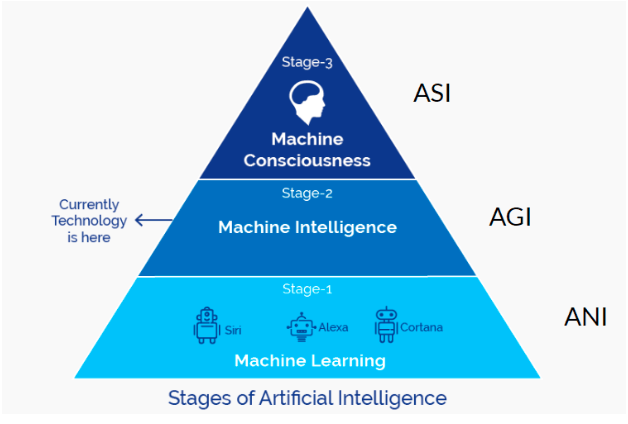
\includegraphics[scale=0.6]{tiposdeai.png}
    \caption{Pirâmide ilustrativa da hierarquia dos diferentes tipos de \ac{ai}}
    \label{piramide}
\end{figure}

%%%%%%%%%%%%%%%%%%%%%%%%%%%%%%%%%%%%%%%%%%%%%%%%%%%%%%%%%%%%%%%%%%%%%%%%%%%%%%%%%%%%%%%%%%%%%%%%%%%%%%%%%%%%%%%%

\chapter{Robôs}
\label{chap.robos}
A \ac{ai} está a desempenhar um papel cada vez mais importante no desenvolvimento de robôs. Esta permite que os robôs percebam e entendam o seu ambiente, tomem decisões e ajam com base nessas decisões.

Uma das principais formas que a \ac{ai} é utilizada em robôs é no desenvolvimento de robôs autónomos. Robôs capazes de operar sem a necessidade de controle humano direto. Usando uma combinação de sensores, câmaras e algoritmos avançados, os robôs autónomos são capazes de navegar no seu ambiente, evitar obstáculos e executar tarefas. Essa tecnologia está a ser usada em uma ampla gama de aplicações, incluindo manufatura, saúde e logística.

Além dos robôs autónomos, a \ac{ai} também está a ser usada para melhorar o desempenho dos robôs em diversas tarefas. Por exemplo, os robôs em ambientes de fabricação geralmente são equipados com sistemas de visão alimentados por \ac{ai} que permitem reconhecer e manipular objetos. Isso pode melhorar a velocidade e a precisão de tarefas como montagem e embalagem.

No geral, o uso de \ac{ai} em robôs está a ajudar a tornar essas máquinas mais capazes e versáteis. À medida que essa tecnologia continua a evoluir, podemos esperar ver robôs ainda mais avançados e sofisticados no futuro.

\section{Robôs Humanoides}
Aprofundando um pouco mais no tema da robótica, deparamos-nos com o uso de \ac{ai} na construção de robôs humanoides.

Um robô humanoide é um tipo de robô projetado para se assemelhar ao corpo humano e seus movimentos. Esses robôs são normalmente construídos com dois braços, duas pernas e uma cabeça, e são capazes de mover e manipular objetos de maneira semelhante à de um humano.

A ideia de criar máquinas semelhantes a humanos existe há séculos, com as primeiras tentativas de robôs humanoides que remontam aos tempos antigos. Por exemplo, os antigos gregos criaram servos mecânicos e autómatos, incluindo o lendário gigante de bronze Talos e os complexos mecanismos de \textit{Antikythera}.

\begin{wrapfigure}{l}{0.25\textwidth}
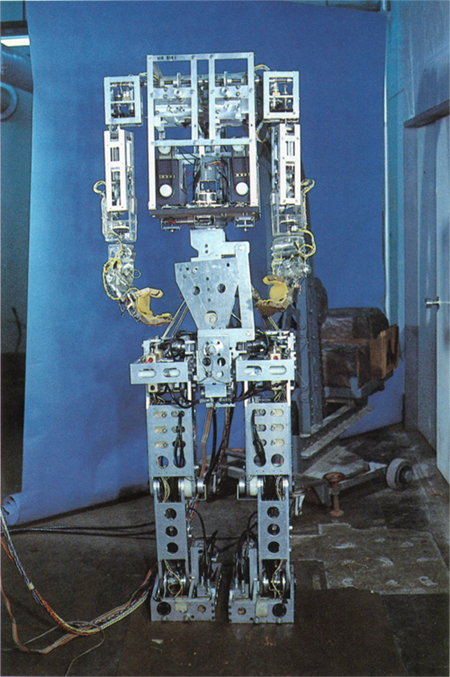
\includegraphics[width=0.9\linewidth]{wabot.png} 
\caption{Wabot1 Primeiro robô antropomórfico em escala humana desenvolvido no mundo}
\label{wabot}
\end{wrapfigure}


Ao longo dos séculos houveram muito mais tentativas de criar robôs humanoides, mas foi no século XX que um progresso significativo foi feito. Na década de 1970, o desenvolvimento de tecnologia avançada de computação e robótica permitiu a criação de robôs humanoides mais sofisticados \cite{wabot}.

Nas últimas décadas, o campo da robótica humanoide continuou a avançar rapidamente, com desenvolvimentos significativos nas áreas de inteligência artificial, aprendizado de máquina e sensores e atuadores avançados. Isso levou à criação de robôs humanoides que são capazes de se mover e funcionar mais como humanos e a uma gama mais ampla de aplicações para essas máquinas.

Os robôs humanoides são frequentemente usados em pesquisa e desenvolvimento, bem como em uma variedade de aplicações, incluindo manufatura, entretenimento e saúde. Eles podem ser usados para tarefas difíceis ou perigosas para humanos executarem, como explorar ambientes perigosos ou realizar cirurgias complexas.

\begin{wrapfigure}{l}{0.25\textwidth}
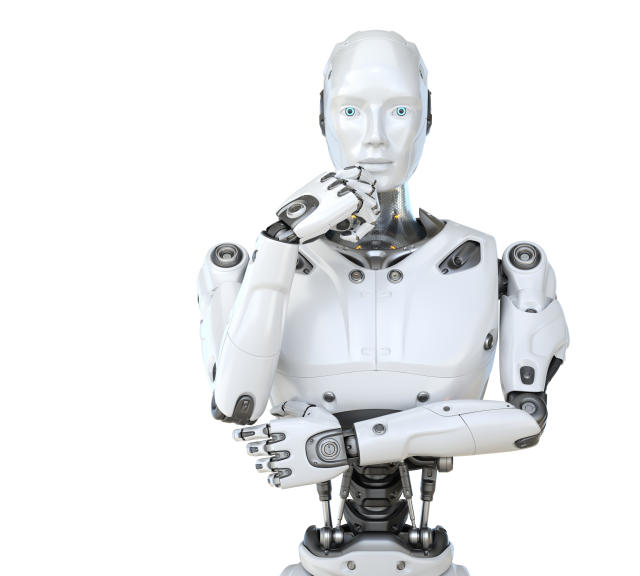
\includegraphics[width=0.9\linewidth]{robo.png} 
\caption{Robô Humanoide}
\label{robohumanoide}
\end{wrapfigure}

Um dos principais desafios no desenvolvimento de robôs humanoides é a necessidade de criar máquinas que sejam capazes de se mover e funcionar da mesma forma que os humanos. Isso requer o uso de sensores, atuadores e algoritmos avançados para permitir que o robô perceba seu ambiente, tome decisões e interaja com objetos e outros humanos.

No geral, os robôs humanoides são uma área empolgante da tecnologia que tem o potencial de revolucionar uma ampla gama de indústrias e aplicações. A história dos robôs humanoides é longa e fascinante, com muitos marcos e desenvolvimentos importantes ao longo do caminho. Os últimos desenvolvimentos no campo são uma grande promessa para o futuro dos robôs humanoides e para as muitas maneiras pelas quais essas máquinas podem ser usadas para melhorar nossas vidas.

São apresentados a seguir alguns exemplos de robôs desta categoria.

\newpage

\subsection{Robô Sophia}

\textit{Sophia} (imagem \ref{sophia}) é um robô humanoide desenvolvido pela empresa Hanson Robotics, sediada em Hong Kong, que tem como objetivo simular expressões faciais. Foi projetado para aprender e adaptar-se ao comportamento do ser humano e trabalhar com estes, sendo capaz de desenvolver conversas simples sobre tópicos predefinidos. O robô \textit{Sophia} foi ativado a 14 de fevereiro de 2016 e é capaz de reproduzir 62 expressões faciais.

\subsection{Robô Optimus}

A empresa Tesla, anunciou em 2021 que está a desenvolver um robô para ser utilizado em tarefas domésticas básicas que causam importuno ao ser humano, como carregar objetos pesados e regar plantas. \textit{Optimus} (imagem \ref{optimus}), também conhecido como \textit{Tesla Bot}, será controlado por uma \ac{ai} que a Tesla está a desenvolver para o sistema avançado de assistência ao motorista usado em seus carros. Este robô é suposto conseguir, numa fase final do seu desenvolvimento, realizar tarefas perigosas e repetitivas, para assistir as pessoas nos trabalhos de produção em fábricas.

\begin{figure}[h]

\begin{subfigure}{0.5\textwidth}
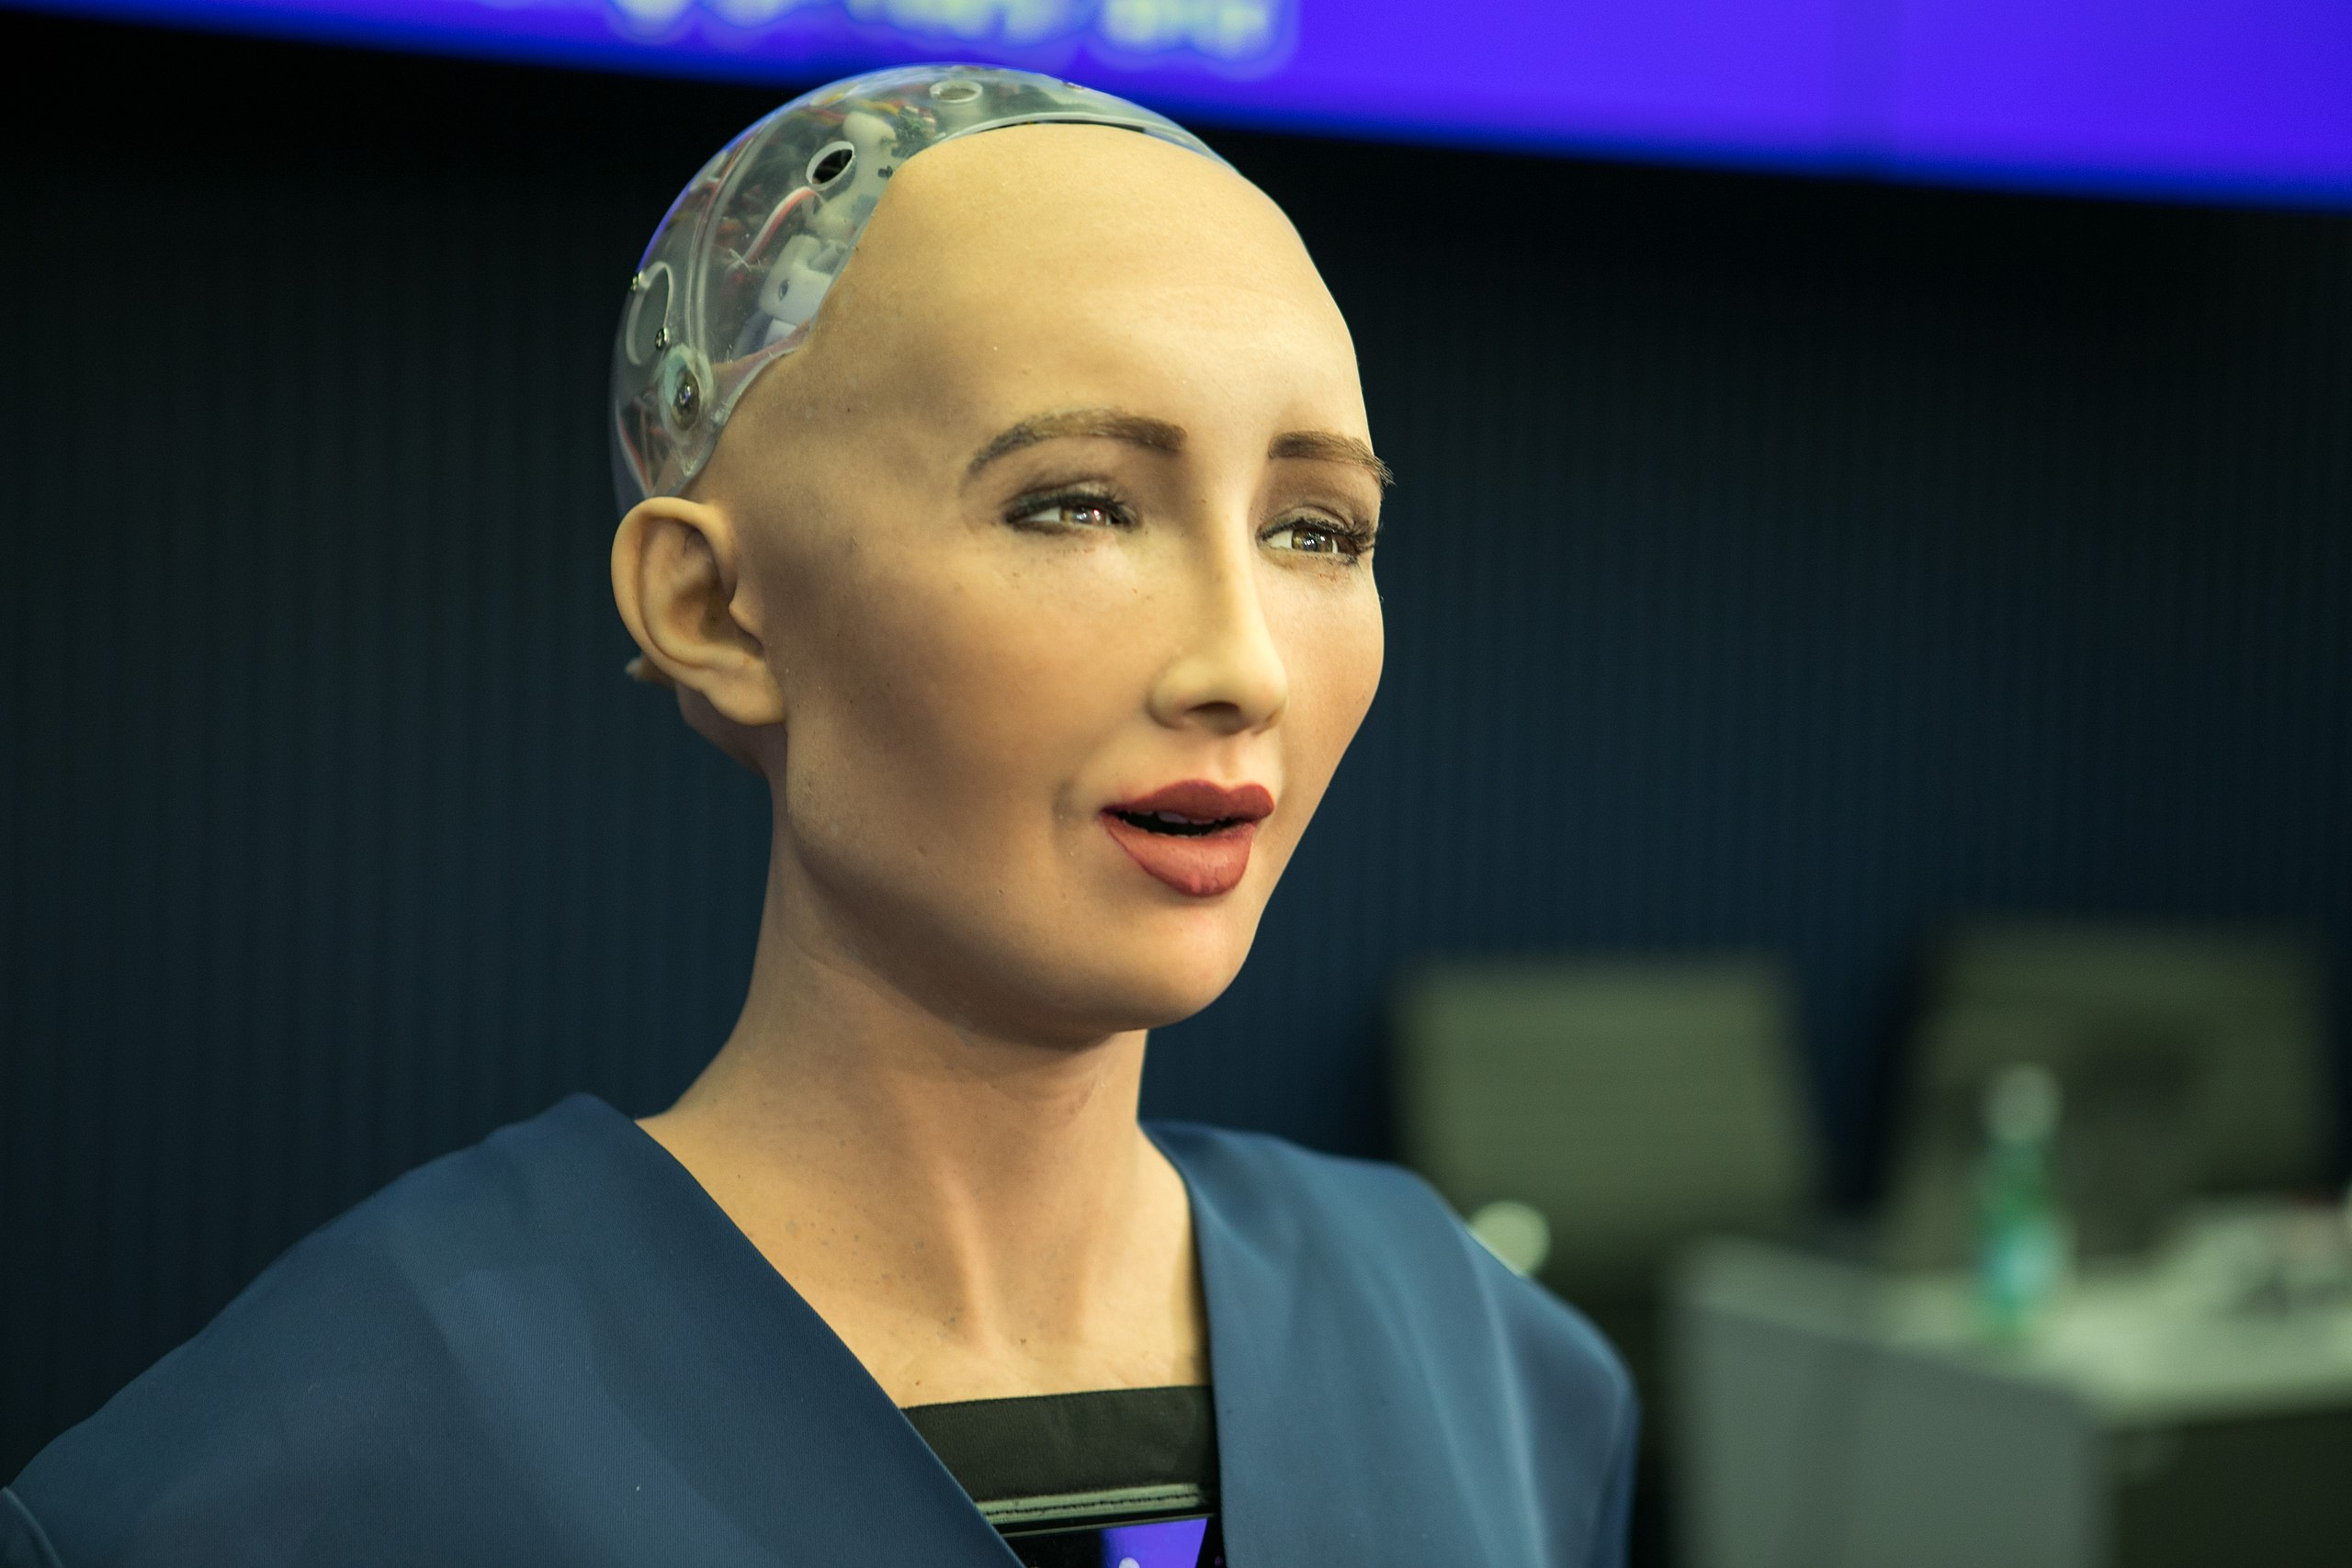
\includegraphics[width=0.9\linewidth, height=4cm]{Sophia.png} 
\caption{Sophia}
\label{sophia}
\end{subfigure}
\begin{subfigure}{0.5\textwidth}
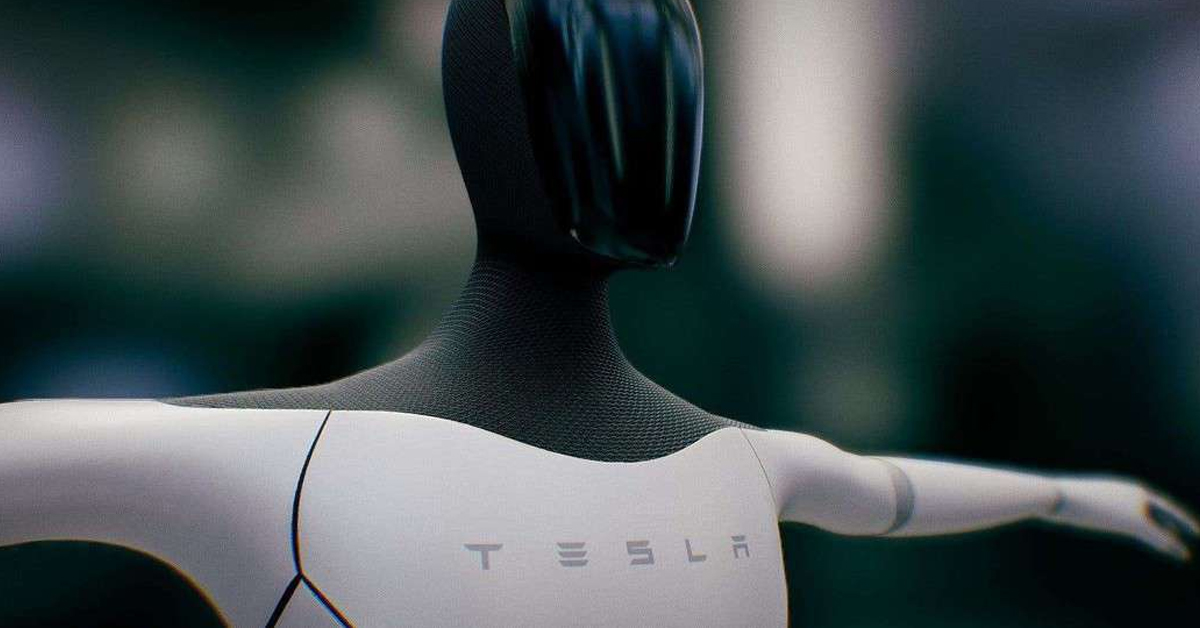
\includegraphics[width=0.9\linewidth, height=4cm]{tesla.png}
\caption{Optimus}
\label{optimus}
\end{subfigure}

\caption{Robôs Humanoides Mais Conhecidos na Atualidade}
\label{Robos}
\end{figure}


%%%%%%%%%%%%%%%%%%%%%%%%%%%%%%%%%%%%%%%%%%%%%%%%%%%%%%%%%%%%%%%%%%%%%%%%%%%%%%%%%%%%%%%%%%%%%%%%%%%%%%%%%%%%%%%%
\chapter{Automóveis}
\label{chap.automoveis}

A \ac{ai} está a desempenhar um papel cada vez mais importante na indústria auto motiva. De carros autónomos a sistemas de veículos inteligentes, a \ac{ai} está a ajudar a tornar a condução mais segura, eficiente e agradável.

Um dos usos mais significativos da \ac{ai} em carros é o desenvolvimento de veículos autónomos. São carros capazes de dirigir sozinhos sem a necessidade de um motorista humano. Usando uma combinação de sensores, câmaras e algoritmos avançados, os carros autónomos são capazes de navegar pelas estradas, evitar obstáculos e tomar decisões em tempo real. Essa tecnologia tem o potencial de reduzir significativamente os acidentes e mortes no trânsito, além de melhorar o fluxo do tráfego e reduzir o congestionamento.

Além dos veículos autónomos, a \ac{ai} também está a ser usada em carros para melhorar a segurança e o desempenho dos veículos. Por exemplo, muitos carros modernos são equipados com sistemas avançados de assistência ao motorista (\ac{adas}) que usam \ac{ai} para monitorar a estrada e fornecer avisos ou assistência ao motorista quando necessário. Esses sistemas podem ajudar os motoristas a evitar colisões, manter distâncias seguras e permanecer em suas faixas.

A \ac{ai} também está a ser usada para aprimorar a experiência de dirigir. Por exemplo, alguns carros são equipados com assistentes virtuais que usam processamento de linguagem natural para entender e responder a comandos de voz. Isso permite que os motoristas controlem várias funções do carro, como o rádio ou o sistema de navegação, sem tirar as mãos do volante.

Uma das grandes utilidades do uso de carros com \ac{ai} desenvolvida é também em questões relacionadas ao envelhecimento da população. Países como o Japão que enfrentam este problema, os carros autónomos com inteligência artificial são um ótimo meio de transporte para idosos e pessoas com deficiências especiais, que apresentam dificuldades em se deslocar e conduzir carros convencionais.

No geral, o uso de \ac{ai} em carros está a ajudar a tornar a direção mais segura, eficiente e agradável. À medida que essa tecnologia continua a evoluir, podemos esperar desenvolvimentos ainda mais empolgantes na indústria auto motiva.

\section{Presença atual no mercado de automóveis que usam \ac{ai}}

Atualmente, o mercado de \ac{ai} na indústria auto motiva está a crescer rapidamente, com muitas empresas a investir de forma pesada no desenvolvimento de tecnologias baseadas em \ac{ai} para carros. De acordo com um relatório recente, o mercado global de \ac{ai} na indústria auto motiva deve atingir US\$ 40,8 bilhões até 2025, com uma taxa composta de crescimento anual de 32,1\% de 2020 a 2025. \cite{aicarros}

Alguns dos principais \textit{players} no mercado de \ac{ai} em carros incluem empresas auto motivas estabelecidas, como Ford, General Motors e Toyota, além de empresas de tecnologia como Google e NVIDIA. Essas empresas estão a investir em uma variedade de tecnologias baseadas em \ac{ai}, incluindo carros autónomos, sistemas avançados de assistência ao motorista (\ac{adas}) e sistemas inteligentes de veículos.

Uma das principais tendências no mercado de \ac{ai} em carros é o crescente desenvolvimento e implementação de carros autónomos. Esses veículos usam uma combinação de sensores, câmaras e algoritmos avançados para navegar pelas estradas e tomar decisões em tempo real, sem a necessidade de um motorista humano. Muitas empresas estão atualmente a trabalhar na tecnologia de carros autónomos, e espera-se que ela se torne mais amplamente disponível nos próximos anos.

Outra tendência no mercado de \ac{ai} em carros é o uso crescente de \ac{ai} em \ac{adas}. Esses sistemas usam \ac{ai} para monitorar a estrada e fornecer avisos ou assistência ao motorista quando necessário. Isso pode ajudar a melhorar a segurança e o desempenho do veículo, e espera-se que se torne mais comum nos próximos anos.

%%%%%%%%%%%%%%%%%%%%%%%%%%%%%%%%%%%%%%%%%%%%%%%%%%%%%%%%%%%%%%%%%%%%%%%%%%%%%%%%%%%%%%%%%%%%%%%%%%%%%%%%%%%%%%%%
\chapter{GitHub Copilot}
\label{chap.github}
Uma das aplicações mais pertinentes de \ac{ai} é no desenvolvimento de ferramentas de auxílio à programação. Uma das ferramentas mais populares é o \textbf{\textit{GitHub Copilot}}, \textit{'Your AI pair programme'}. De uma forma resumida, esta ferramenta dá ao programador sugestões de código para preenchimento automático, permitindo assim poupar muito tempo. Esta \ac{ai} é até capaz de produzir código de funções inteiras de forma completamente autónoma.

\hfill

\begin{figure}[h]
    \centering
    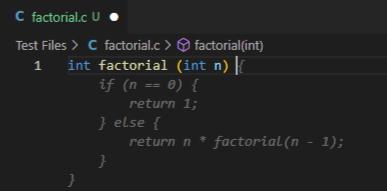
\includegraphics{factorial.png}
    \caption{Função para calcular o fatorial de um número em C}
    \label{factorial1}
\end{figure}

Como podemos ver na imagem \ref{factorial1}, a \ac{ai} escreveu o código todo necessário para a função ser implementada com sucesso, bastando apenas ao programador escrever o nome da função.

Esta ferramenta, não substitui no entanto uma pessoa, não sendo ainda capaz de escrever um programa completamente de forma autónoma. Com o desenvolvimento da tecnologia é provável que num futuro próximo isto venha a ser possível.
%%%%%%%%%%%%%%%%%%%%%%%%%%%%%%%%%%%%%%%%%%%%%%%%%%%%%%%%%%%%%%%%%%%%%%%%%%%%%%%%%%%%%%%%%%%%%%%%%%%%%%%%%%%%%%%%
\chapter{Xadrez}
\label{chap.xadrez}

\section{O que é uma \textit{Chess Engine}}

\textit{Chess Engines} (\ac{ce}) são programas de computador projetados para jogar o jogo de xadrez. Esses programas usam algoritmos avançados e técnicas de inteligência artificial para analisar o tabuleiro de xadrez e tomar decisões sobre quais jogadas fazer.

Os mecanismos de xadrez são uma ferramenta importante para os jogadores de xadrez, pois podem fornecer informações e análises valiosas que podem ajudar os jogadores a melhorar o seu jogo. Muitas \ac{ce} estão disponíveis, variando de programas simples que fornecem análises básicas a mecanismos altamente sofisticados capazes de competir nos níveis mais altos do jogo.

Uma das principais características das \ac{ce} é sua capacidade de pesquisar um grande número de movimentos e variações possíveis em um curto período de tempo. Isso permite que elas analisem posições complexas e avaliem diferentes linhas de jogo, proporcionando aos jogadores uma compreensão mais profunda da posição no tabuleiro.

As \ac{ce} também podem ser usadas para ajudar os jogadores a praticar e melhorar suas habilidades. Muitos mecanismos incluem recursos de treinamento e quebra-cabeças táticos, que podem ajudar os jogadores a desenvolver o seu pensamento estratégico e habilidades táticas. Alguns motores também incluem recursos que permitem aos jogadores jogar contra o motor, proporcionando um adversário desafiador para jogadores de todos os níveis.

No geral, as \ac{ce} são uma ferramenta importante para jogadores de xadrez, fornecendo análise valiosa e recursos de treinamento que podem ajudar os jogadores a melhorar o seu nível de jogo. À medida que a tecnologia continua a evoluir, podemos esperar ver \ac{ce} ainda mais avançadas e sofisticadas no futuro.

\section{Torneios de \ac{ce}}

Existem vários campeonatos de \ac{ce} que são realizados a cada ano, incluindo o \ac{tcec} e o \ac{ccc}. Estes campeonatos são organizados por várias organizações e sites de xadrez e são projetados para determinar a \ac{ce} mais forte do mundo.

O \ac{tcec} é um prestigioso campeonato anual de \ac{ce} que acontece desde 2010. É organizado pelo site Chessdom e apresenta um formato de vários estágios com uma variedade de controles de tempo e livros de abertura. O vencedor do \ac{tcec} é considerado \ac{ce} mais forte do mundo.

O \ac{ccc} é outro campeonato anual de \ac{ce}, organizado pela \ac{icga}. O \ac{ccc} apresenta um formato round-robin, com motores competindo entre si em uma série de jogos. O vencedor do \ac{ccc} também é considerado uma das \ac{ce} mais fortes do mundo.

No geral, os campeonatos de \ac{ce} são eventos importantes no mundo do xadrez, fornecendo uma plataforma para os melhores motores competirem e determinarem o mais forte. Esses campeonatos são acompanhados de perto pelos entusiastas do xadrez e podem fornecer informações valiosas sobre o estado da arte da tecnologia de \ac{ce}.

Um dos sites mais populares do mundo de xadrez é o \href{http://www.chess.com}{\textbf{Chess.com}}, onde é possível assistir em tempo real a um dos campeonatos de \ac{ce} mais prestigiados \cite{chessenginechampionship}.

\section{Site mais popular de Xadrez online onde são aplicadas \ac{ce}}

Chess.com é um site popular e uma plataforma online para jogar e aprender xadrez. O site foi fundado em 2005 e está sediado em San Francisco, Califórnia. Ele oferece uma variedade de recursos e ferramentas para jogadores de xadrez de todos os níveis, de iniciantes a grandes mestres.

Uma das principais características do Chess.com é sua plataforma de xadrez online, que permite aos usuários jogar contra outros jogadores de todo o mundo. A plataforma oferece uma variedade de modos de jogo, incluindo xadrez padrão, blitz e bala, bem como variantes de xadrez como Crazyhouse e Chess960.

Além da sua plataforma de xadrez online, o Chess.com também oferece uma variedade de ferramentas de aprendizado e treinamento para jogadores de xadrez. Isso inclui vídeos instrutivos, aulas interativas e quebra-cabeças táticos, bem como acesso a uma grande comunidade de jogadores de xadrez que podem fornecer conselhos e suporte e claro, a integração de \ac{ce} como auxiliar em todos estes recursos.

O Chess.com também hospeda torneios de xadrez online, com jogadores de todo o mundo competindo por prémios em dinheiro e outras recompensas. O site também oferece uma variedade de ferramentas e recursos para clubes e organizações de xadrez, incluindo ferramentas para gerir associações e organizar eventos.

No geral, o Chess.com é um destino popular e respeitado para jogadores de xadrez de todos os níveis. Sua combinação de xadrez online, ferramentas de aprendizado e recursos da comunidade tornam-no um recurso valioso para quem quer melhorar suas habilidades no xadrez e aproveitar o jogo.

\section{\textit{Chess Engines} mais populares \cite{chessenginesmaispopulares}}
\begin{itemize}
        \item \textbf{Stockfish}
        \item \textbf{AlphaZero} 
        \item \textbf{Leela Chess Zero} 
        \item \textbf{Komodo Chess}
        \item \textbf{Deep Blue}
        \item \textbf{Shredder Chess}
        \item \textbf{Fritz}
        \item \textbf{Rybka}
        \item \textbf{Houdini Chess}
        \item \textbf{HIARCS}
\end{itemize}
\section{Comparação entre uma \ac{ce} e os melhores jogadores de Xadrez do mundo}

\begin{table}[h!]
\centering
\begin{tabular}{  |p{3cm}|p{3cm}|  }
\hline
\multicolumn{2}{|c|}{Fide Rating} \\
\hline
Players & Fide Elo Points\\
\hline
Stockfish & 3620 \\
Magnus Carlsen & 2859  \\
Liren Ding & 2811 \\
Ian Nepomniatchi & 2793 \\
Alireza Firouzja & 2785 \\
Hikaru Nakamura & 2768  \\
Fabiano Caruana & 2766  \\
\hline
\end{tabular}
\end{table}

Nas últimas duas décadas, as \ac{ce} excederam por completo as capacidades dos seres humanos, como podemos ver pela tabela \cite{chess}.


\newpage

\section{Jogo entre uma \textit{Chess Engine} e um \textit{Grand Master} \cite{kasparov}, a primeira vez que uma \ac{ce} derrota o campeão mundial}
{\centering{\Large Deep Blue(white)-Kasparov(black) \normalsize}}\\
\newchessgame
\mainline{1.e4 c5 2.c3 d5 3.exd5 Qxd5 4.d4 Nf6 5.Nf3 Bg4 6.Be2 e6 7.h3 Bh5 8.O-O Nc6 9.Be3 cxd4 10.cxd4 Bb4 11.a3 Ba5 12.Nc3 Qd6 13.Nb5 Qe7 14.Ne5 Bxe2 15.Qxe2 O-O 16.Rac1 Rac8 17.Bg5 Bb6 18.Bxf6 gxf6 19.Nc4 Rfd8 20.Nxb6 axb6 21.Rfd1 f5 22.Qe3 Qf6 23.d5 Rxd5 24.Rxd5 exd5 25.b3 Kh8 26.Qxb6 Rg8 27.Qc5 d4 28.Nd6 f4 29.Nxb7 Ne5 30.Qd5 f3 31.g3 Nd3 32.Rc7 Re8 33.Nd6 Re1+ 34.Kh2 Nxf2 35.Nxf7+ Kg7 36.Ng5+ Kh6 37.Rxh7+}\par
\chessboard[showmover=false]

\epigraph{It's 1997, and the world watches in disbelief as GM Garry Kasparov, arguably the best chess player in history, loses a match against a computer. The era of chess engines has started, changing the game's landscape forever.} {\textit{Chess.com \cite{chessenginesmaispopulares}}}

\newpage

\section{O futuro das \textit{Chess Engines}}

O futuro dos motores de xadrez provavelmente será caracterizado por avanços contínuos em tecnologia e inteligência artificial. À medida que as capacidades dos mecanismos de xadrez continuam a melhorar, eles se tornarão oponentes ainda mais fortes e desafiadores para os jogadores humanos.

Uma das principais tendências no futuro dos mecanismos de xadrez é o uso crescente de aprendizado de máquina e algoritmos de aprendizado profundo. Esses algoritmos permitem que os mecanismos de xadrez aprendam e melhorem com o tempo, analisando grandes quantidades de dados e identificando padrões e tendências no jogo. Isso permitirá que os mecanismos de xadrez se tornem ainda mais sofisticados e capazes de tomar decisões estratégicas a par dos melhores jogadores humanos.

Outra tendência no futuro dos motores de xadrez é o uso crescente de computação em nuvem e sistemas distribuídos. Isso permitirá que os mecanismos de xadrez aproveitem o poder de muitos computadores trabalhando juntos, permitindo que eles analisem e avaliem mais posições e variações em um período de tempo menor. Isso tornará os mecanismos de xadrez ainda mais poderosos e desafiadores para os jogadores humanos.

No geral, o futuro dos mecanismos de xadrez provavelmente será de crescimento e desenvolvimento contínuos, à medida que a tecnologia e a inteligência artificial continuam avançando.


%%%%%%%%%%%%%%%%%%%%%%%%%%%%%%%%%%%%%%%%%%%%%%%%%%%%%%%%%%%%%%%%%%%%%%%%%%%%%%%%%%%%%%%%%%%%%%%%%%%%%%%%%%%%%%%%
\chapter{Perigos da AI}
\label{chap.perigos}

Enquanto \ac{ai} apresenta potencial para trazer muitos benefícios, esta também carrega consigo alguns riscos e perigos. Uma das maiores preocupações é o potencial uso da \ac{ai} de formas maliciosas, como por exemplo no desenvolvimento de armas autónomas ou em cyber ataques.

Outra grande preocupação é a possibilidade da \ac{ai} causar o aumento do desemprego, visto esta substituir o ser humano nas tarefas que este tem de realizar. Em muitas áreas poderá haver fortes perdas de emprego, podendo isto levar a uma disrupção na economia. Assim que os sistemas de \ac{ai} se tornem mais avançados e estes consigam ser capazes de desempenhar tarefas que atualmente são realizadas por seres humanos, vai haver desemprego em larga escala. 

Adicionalmente, há preocupações sobre \ac{ai} poder tomar decisões que têm consequências negativas. Por exemplo, um veículo automático pode tomar a decisão de se desviar de um obstáculo, apenas para causar um acidente ainda pior durante o processo. Há também a probabilidade de sistemas \ac{ai} serem enviesados, quer seja através dos dados ou dos algoritmos usados para o treino dos mesmos.
\begin{wrapfigure}{l}{0.25\textwidth}
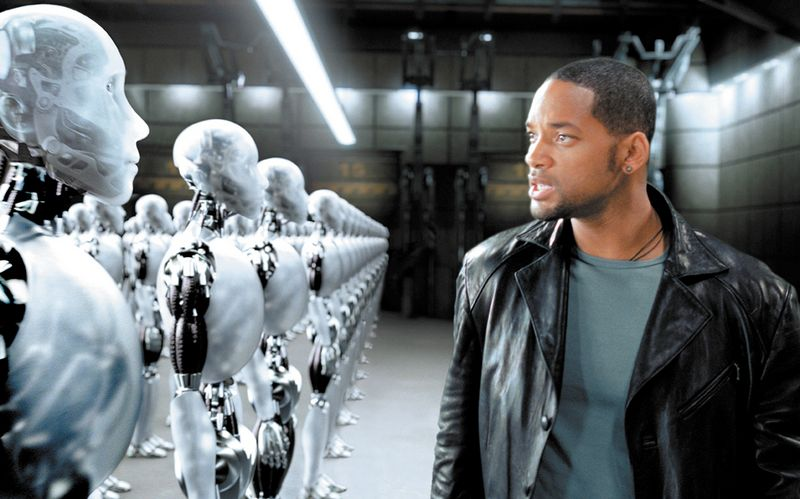
\includegraphics[width=0.9\linewidth]{irobot.png} 
\caption{I, Robot}
\label{i,robot}
\end{wrapfigure}
Vários filmes foram feitos com o tema \ac{ai}. 
Um dos mais aclamados pelas críticas e mais reconhecidos internacionalmente é o filme "I, Robot" protagonizado por Will Smith, que pretende mostrar e dar ênfase aos perigos da \ac{ai}. O filme tem lugar num futuro onde os robôs são dominantes, parte do quotidiano das pessoas. Este filme de ficção científica explora o tema inteligência artificial e as consequências negativas da criação e desenvolvimento da tecnologia, levantando questões sobre o papel da \ac{ai} na sociedade e o que pode vir a acontecer se as máquinas se tornarem mais inteligentes do que os seres humanos.


%%%%%%%%%%%%%%%%%%%%%%%%%%%%%%%%%%%%%%%%%%%%%%%%%%%%%%%%%%%%%%%%%%%%%%%%%%%%%%%%%%%%%%%%%%%%%%%%%%%%%%%%%%%%%%%%
\chapter{Conclusão}
\label{chap.conclusao}
Em suma, o desenvolvimento de \ac{ai} tem muito potencial para revolucionar vários aspetos das nossas vidas. Desde carros capazes de se deslocar de forma autónoma em modo piloto automático, casas inteligentes controladas por robôs que desempenham as tarefas domésticas do dia a dia, até sistemas médicos de análise e diagnóstico avançados. A \ac{ai} é já muito usada atualmente numa alta variedade de aplicações. No entanto, o rápido crescimento da \ac{ai} trás problemas que têm de ser medidos de forma cautelosa. É importante que cientistas, e a sociedade em geral como um todo, considerem cuidadosamente os perigos e benefícios da \ac{ai} e tomem medidas para garantir que esta tecnologia é desenvolvida e usada de uma forma responsável e ética, minimizando as consequências negativas do seu uso. Com planeamento cuidadoso e com consideração, podemos aproveitar e extrair o poder da \ac{ai} para melhorar as nossas vidas e criar um futuro próspero para todos.
%%%%%%%%%%%%%%%%%%%%%%%%%%%%%%%%%%%%%%%%%%%%%%%%%%%%%%%%%%%%%%%%%%%%%%%%%%%%%%%%%%%%%%%%%%%%%%%%%%%%%%%%%%%%%%%%
\chapter*{Contribuições dos autores}
O trabalho foi realizado pelo aluno \ac{bm}.


Nome do repositório: infor2022-ap-g12

\vspace{10pt}
\textbf{Percentagem de contribuição de cada autor.}\\

\autores : 100\%
%%%%%%%%%%%%%%%%%%%%%%%%%%%%%%%%%%%%%%%%%%%%%%%%%%%%%%%%%%%%%%%%%%%%%%%%%%%%%%%%%%%%%%%%%%%%%%%%%%%%%%%%%%%%%%%%
%%%%%%%%%%%%%%%%%%%%%%%%%%%%%%%%%
\chapter*{Acrónimos}
\begin{acronym}
\acro{ua}[UA]{Universidade de Aveiro}
\acro{leci}[LECI]{Licenciatura em Engenharia de Computadores e Informática}
\acro{glisc}[GLISC]{Grey Literature International Steering Committee}
\acro{ai}[AI]{Artificial Intelligence}
\acro{ani}[ANI]{Inteligência Artificial Limita}
\acro{agi}[AGI]{Inteligência Artificial Geral}
\acro{asi}[ASI]{Super-inteligência}
\acro{adas}[ADAS]{Advanced Driver Assistance Systems}
\acro{ce}[CE]{Chess Engine}
\acro{tcec}[TCEC]{Top Chess Engine Championship}
\acro{ccc}[CCC]{Computer Chess Championship}
\acro{icga}[ICGA]{International Computer Games Association}
\acro{bm}[BM]{Bernardo Marujo}
\end{acronym}


%%%%%%%%%%%%%%%%%%%%%%%%%%%%%%%%%
\printbibliography

\end{document}
